% !TEX program = xelatex
% 光遗传学与视觉功能恢复 · 按材料分组版（22 问 / 52 分）
% 编译：xelatex -interaction=nonstopmode -halt-on-error 本文件（跑两遍）
\documentclass[UTF8,a4paper,11pt]{ctexart}

\usepackage{geometry}
\geometry{left=1.9cm,right=1.9cm,top=2.3cm,bottom=2.3cm}
\usepackage{graphicx}
\usepackage{amsmath,amssymb}
\usepackage{booktabs}
\usepackage{longtable}
\usepackage{array}
\usepackage{enumitem}
\usepackage{xcolor}
\usepackage{caption}
\usepackage{float}
\usepackage{titlesec}
\usepackage{fancyhdr}
\usepackage{tcolorbox}
\tcbuselibrary{skins,breakable}
\usepackage[hidelinks]{hyperref}

\graphicspath{{../命题图/}{../../Resources/Downloads/原图-光遗传学视觉恢复/}}

\definecolor{deepblue}{HTML}{1F4E79}
\definecolor{deepred}{HTML}{C00000}
\definecolor{deepgreen}{HTML}{2E7D32}

\captionsetup{font=small,labelfont=bf,skip=4pt}
\titleformat{\section}{\Large\bfseries\color{deepblue}}{\thesection}{0.6em}{}
\pagestyle{fancy}
\fancyhf{}
\fancyhead[L]{\small 光遗传学与视觉功能恢复 · 按材料分组版（52 分）}
\fancyhead[R]{\small\thepage}

\newcommand{\pt}[1]{\textbf{（#1分）}}
\newcommand{\lv}[1]{{\small\color{deepgreen}［#1］}}
\newcommand{\key}[1]{\textbf{\color{deepred}#1}}
\newcommand{\tian}[1]{\underline{\hspace{#1}}}
\newcommand{\choice}[1]{\par\smallskip\noindent #1\par}

\newtcolorbox{matbox}[1]{colback=blue!4,colframe=deepblue,boxrule=0.9pt,
  arc=2pt,left=6pt,right=6pt,top=5pt,bottom=5pt,
  title={\bfseries #1},fonttitle=\normalsize\color{white},
  coltitle=white,colbacktitle=deepblue,breakable}
\newtcolorbox{qbox}{colback=deepgreen!5,colframe=deepgreen,boxrule=0.7pt,
  arc=2pt,left=6pt,right=6pt,top=4pt,bottom=4pt,breakable,
  before skip=6pt,after skip=6pt}

\title{\bfseries 光遗传学与视网膜退化性疾病的视觉功能恢复\\[5pt]
\large 按材料分组版\quad 22 问 / 52 分}
\author{}\date{2026-10-06}

\begin{document}
\maketitle
\thispagestyle{fancy}

\begin{center}
\fbox{\parbox{0.95\textwidth}{\small
\textbf{组卷方式}：\textbf{每段材料之后紧跟由该材料衍生的设问}，逐段推进——
材料一（RP 与视觉通路）→ 材料二（ChR2 本体）→ 材料三（天然 ChR2 的缺陷与基因工程/蛋白质工程改造）→ 材料四（AAV 载体导入与靶向表达）→ 材料五（视动反应评价）→ 综合。
科研事实取自 Pan et al. 2014、Lu et al. 2016、Lu et al. 2018 三篇开放获取论文；专业名词均在材料或表注中解释，不需事先记忆；标"\key{命题简化}"的数据为命题需要而设定，趋势依原论文改写。
}}
\end{center}

\section*{命题说明}
\addcontentsline{toc}{section}{命题说明}

\begin{table}[H]
\centering\small
\begin{tabular}{@{}llcccc@{}}
\toprule
\textbf{题号} & \textbf{题型} & \textbf{考查落点} & \textbf{难度} & \textbf{分值} & \textbf{材料} \\
\midrule
Q1 & 单选 & 感光细胞的功能 & 基础 & 2 & 一 \\
Q2 & 编号排序 & 正常的光感受与传递通路 & 基础 & 2 & 一 \\
Q3 & 多选 & 视网膜各级细胞的功能分工 & 基础 & 2 & 一 \\
Q4 & 多选 & 神经调节基础（传导、传递、视神经） & 基础 & 2 & 一 \\
Q5 & 简答 & RP 患者视力下降的原因分析 & 中等 & 3 & 一 \\
Q6 & 多选 & 通道蛋白与离子跨膜运输 & 中等 & 2 & 二 \\
Q7 & 多选 & 反射与反射弧的完整性 & 中等 & 2 & 二 \\
Q8 & 简答 & 为什么选择"残存的视网膜细胞"作靶细胞 & 中等 & 3 & 二 \\
Q9 & 简答 & 导入后的作用（光信号→电信号）与意义 & 中等 & 3 & 二 \\
Q10 & 多选 & 治疗性质辨析（功能补偿非根治） & 中等 & 2 & 二 \\
Q11 & 单选 & 变异类型的判断（基因突变） & 基础 & 2 & 三 \\
Q12 & 简答 & 通过改造基因来改造蛋白质的道理（蛋白质工程） & 中等 & 2 & 三 \\
Q13 & 编号排序 & 据表比较被弱光激活的能力 & 基础 & 2 & 三 \\
Q14 & 多选 & 被弱光激活的能力与恢复时间的关系 & 中等 & 2 & 三 \\
Q15 & 简答 & 多指标权衡（优势与局限） & 拔高 & 3 & 三 \\
Q16 & 编号选填+简答 & 据表选择方案并说明理由 & 中等 & 3 & 四 \\
Q17 & 多选 & 载体与调控元件的功能 & 中等 & 2 & 四 \\
Q18 & 简答 & 表达量 ≠ 功能（层次差异） & 拔高 & 3 & 四 \\
Q19 & 单选 & 据表判断视觉功能恢复最好者 & 中等 & 2 & 五 \\
Q20 & 多选 & 对照与评价指标 & 拔高 & 2 & 五 \\
Q21 & 简答 & 实验变量分析＋对照的作用 & 中等 & 3 & 五 \\
Q22 & 简答·开放 & 综合方案与依据 & 拔高 & 3 & 综合 \\
\midrule
\multicolumn{4}{r}{\textbf{合计}} & \textbf{52} & \\
\bottomrule
\end{tabular}
\end{table}

\noindent\textbf{题型分布}：单选 3、多选 8、编号选填 1、编号排序 2，客观题共 14 问 27 分；简答与分析 8 问 25 分。
\textbf{难度分层}：基础 14 分；中等 23 分；拔高 15 分。

\section{材料一\quad RP 与视觉信号通路}
\addcontentsline{toc}{section}{材料一：RP 与视觉信号通路}

\begin{matbox}{材料一\quad RP 与视觉信号通路}
视网膜像一台"光信号转换器"，把进入眼内的光变成神经信号送往大脑。视网膜中的\textbf{感光细胞}（视杆细胞与视锥细胞）感受光刺激，并把光信号转变为电信号；信号随后经\textbf{双极细胞}传到\textbf{神经节细胞}，后者的轴突汇聚成\textbf{视神经}，把信号送往大脑皮层的\textbf{视觉中枢}，最终形成视觉（图1）。

视网膜色素变性（RP）是一类由基因突变引起的遗传性眼病。患者的\textbf{感光细胞逐渐死亡}，而内层的双极细胞与神经节细胞大多仍然存活。这类患者即使眼球结构、视神经和视觉中枢都没有明显损伤，视力仍会不断下降，直至失明。
\end{matbox}

\begin{figure}[H]
\centering
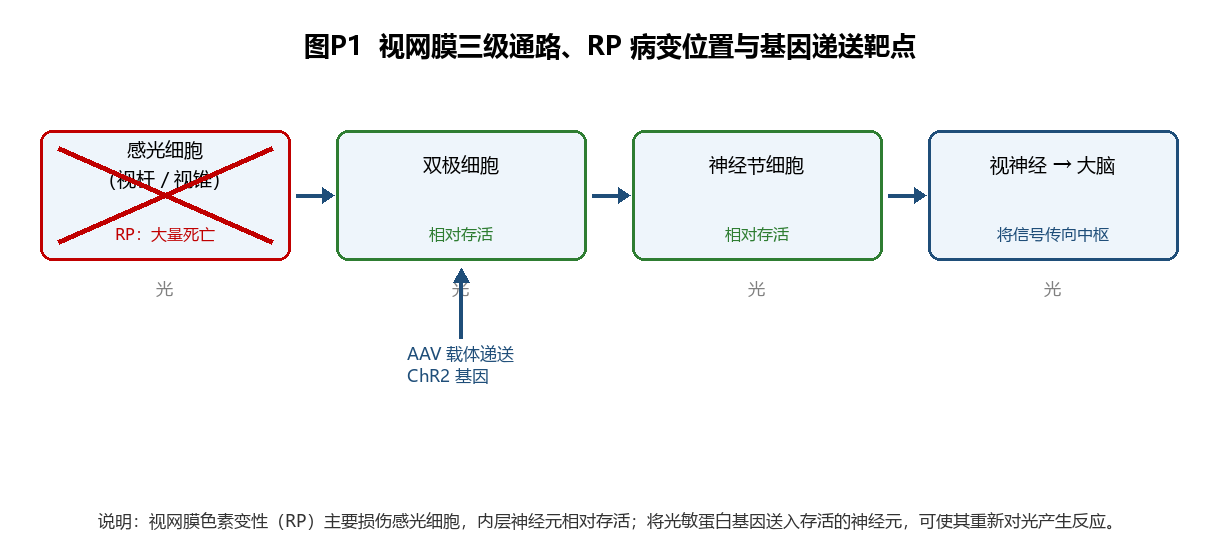
\includegraphics[width=0.6\textwidth]{P1_视网膜三级通路与病变.png}
\caption{图1\quad 视网膜三级细胞通路、RP 的主要受损环节与治疗靶点（简化示意图）}
\end{figure}

\begin{qbox}
\noindent\textbf{\color{deepgreen}第 1—5 问（据材料一作答）}
\begin{enumerate}[leftmargin=2.2em,itemsep=5pt]
\item \lv{单选} \pt{2} 在正常的视网膜中，把光信号转变为电信号的细胞是（\quad）\\
\choice{A. 感光细胞 \quad B. 双极细胞 \quad C. 神经节细胞 \quad D. 视神经}

\item \lv{编号排序} \pt{2} 用编号和箭头（→）表示正常情况下光信号从进入眼球到形成视觉所经过的途径：\\
\choice{① 感光细胞 \quad ② 双极细胞 \quad ③ 视神经 \quad ④ 神经节细胞 \quad ⑤ 大脑皮层视觉中枢\\
答：\tian{7.4cm}}

\item \lv{多选} \pt{2} 据材料一与图1，关于视网膜各级细胞的功能，下列说法正确的有（\quad）（错选得 0 分）\\
\choice{A. 感光细胞能感受光刺激，并把光信号转变为电信号\\
B. 双极细胞接受感光细胞的信号，并把它传给神经节细胞\\
C. 神经节细胞的轴突汇聚成视神经，把信号传向大脑\\
D. 视网膜只起"传递"作用，视觉信号的全部加工都发生在眼球之外}

\item \lv{多选} \pt{2} 结合材料与所学知识，关于视觉信号的传递，下列说法正确的有（\quad）（错选得 0 分）\\
\choice{A. 兴奋在神经纤维上以电信号（神经冲动）的形式传导\\
B. 兴奋从一个神经元传到另一个神经元要通过突触，且传递是单向的\\
C. 视神经由神经节细胞的轴突构成，属于把信号传向中枢的传入神经\\
D. 只要视网膜中的细胞产生了兴奋，动物就一定能"看见"物体}

\item \lv{中等} \pt{3} 结合材料与图1，分析 RP 患者视力下降的原因。\tian{0.48\textwidth}
\end{enumerate}
\end{qbox}

\section{材料二\quad ChR2：让存活的视网膜细胞重新"感光"}
\addcontentsline{toc}{section}{材料二：ChR2}

\begin{matbox}{材料二\quad ChR2：让存活的视网膜细胞重新"感光"}
研究者尝试用\textbf{光遗传学}方法恢复视觉。他们使用一种来自单细胞藻类的光敏蛋白——\textbf{通道视紫红质（ChR2）}：它由 ChR2 基因编码，在细胞膜上形成一种\textbf{受光控制的离子通道}。蓝光照射时通道开放，离子顺浓度梯度通过通道进入细胞，使细胞膜电位发生改变，细胞由此产生电信号——也就是说，ChR2 把"\textbf{有没有光}"这一信息转变成了细胞内的\textbf{电信号}。

那么，为什么要把 ChR2 基因导入"\textbf{残存的视网膜细胞}"？因为 RP 患者的感光细胞已经大量死亡，无法再感受光；而位于其下游的双极细胞、神经节细胞大多存活，视觉信号本来也正是沿"双极细胞 → 神经节细胞 → 视神经 → 大脑皮层视觉中枢"这条通路传递的。把 ChR2 导入这些存活的细胞后，光照可以直接使它们产生电信号，从而\textbf{绕过已经死亡的感光细胞}，让信号沿原有通路继续传向大脑。
\end{matbox}

\begin{qbox}
\noindent\textbf{\color{deepgreen}第 6—10 问（据材料二作答）}
\begin{enumerate}[leftmargin=2.2em,itemsep=5pt,start=6]
\item \lv{多选} \pt{2} 关于 ChR2 蛋白与离子的跨膜运输，下列说法正确的有（\quad）（错选得 0 分）\\
\choice{A. ChR2 分布在细胞膜上，属于膜蛋白中的通道蛋白\\
B. 蓝光使 ChR2 通道开放后，离子顺浓度梯度通过该通道进入细胞，这一过程不消耗细胞代谢产生的能量\\
C. 通道蛋白对被运输的物质具有选择性，一般只允许特定种类（或特定电荷）的离子通过\\
D. 离子通过 ChR2 进入细胞的方式属于主动运输，因为它需要通道蛋白的协助}

\item \lv{多选} \pt{2} 关于反射与反射弧，下列说法正确的有（\quad）（错选得 0 分）\\
\choice{A. 反射活动的完成必须以完整的反射弧为基础\\
B. 反射弧通常包括感受器、传入神经、神经中枢、传出神经和效应器五部分\\
C. 若某小鼠的视神经已完全损伤，即使其视网膜细胞表达了 ChR2，该技术也不能使它恢复视觉\\
D. 只要效应器表现出反应，就说明该动物发生了反射}

\item \lv{中等} \pt{3} 研究者为什么要把 ChR2 基因导入"\textbf{残存的视网膜细胞}"，而不导入其他细胞？\tian{0.48\textwidth}

\item \lv{中等} \pt{3} 导入 ChR2 基因后，这些原本不能感受光的神经细胞获得了什么能力？请结合 ChR2 的作用说明；这对恢复视觉有什么意义？\tian{0.48\textwidth}

\item \lv{多选} \pt{2} 结合材料，关于 RP 与光遗传学治疗，下列说法合理的有（\quad）（错选得 0 分）\\
\choice{A. RP 患者感光细胞大量死亡，而双极细胞与神经节细胞大多存活\\
B. 把 ChR2 基因导入残存神经细胞后，这些细胞在蓝光照射下可产生电位变化\\
C. 光遗传学治疗从根本上修复了患者致病的基因，因此可治愈 RP\\
D. 治疗后视觉信号仍需经神经节细胞传至大脑皮层视觉中枢才能形成视觉}
\end{enumerate}
\end{qbox}

\section{材料三\quad 天然 ChR2 的不足与蛋白质工程改造}
\addcontentsline{toc}{section}{材料三：天然 ChR2 的不足与蛋白质工程改造}

\begin{matbox}{材料三\quad 天然 ChR2 的不足与蛋白质工程改造}
天然 ChR2 有一个明显的不足：它需要在\textbf{较强}的光下才能被有效激活，而患者所处的环境光往往较弱。要解决这个问题，必须改变 ChR2 蛋白本身的性质。

蛋白质的功能由其\textbf{结构}决定，而蛋白质的结构又由\textbf{基因}（碱基序列）决定。于是研究者采用\textbf{蛋白质工程}的思路：先分析 ChR2 蛋白结构与功能的关系，找出与"对光的敏感程度"有关的关键位置，再通过\textbf{改造基因}——即改变 ChR2 基因中特定位置的碱基序列——来改变蛋白质中相应的氨基酸，从而获得功能更优的 ChR2 蛋白。这样改造得到的蛋白称为\textbf{突变体}。研究者获得了三种突变体，并比较了它们的性能（表1）。
\end{matbox}

\begin{table}[H]
\centering\small
\caption*{\textbf{表1}\quad ChR2 及其突变体的性能比较（\key{命题简化}数据）}
\begin{tabular}{@{}lccc@{}}
\toprule
\textbf{变体} & \textbf{引起光响应所需的最低光强} & \textbf{光照停止后恢复到静息所需时间} & \textbf{在快速闪烁光下的响应} \\
\midrule
wt-ChR2（未改造） & 12 & 短 & 好 \\
M1（ChR2-L132C） & 5 & 中 & 中 \\
M2（ChR2-L132C/T159C） & 2 & 长 & 差 \\
M3（ChR2-L132C/T159S） & 3 & 很长 & 很差 \\
\bottomrule
\end{tabular}

\smallskip
\parbox{0.94\textwidth}{\footnotesize 注："引起光响应所需的最低光强"数值越小，表示细胞在越弱的光下即可被激活；"恢复到静息所需时间"越长，表示细胞在光照停止后越难迅速恢复，对随时间快速变化的光信号跟随能力越弱。数据为命题简化，趋势依据 Pan et al., 2014 改写。}
\end{table}

\begin{qbox}
\noindent\textbf{\color{deepgreen}第 11—15 问（据材料三作答）}
\begin{enumerate}[leftmargin=2.2em,itemsep=5pt,start=11]
\item \lv{单选} \pt{2} 研究者改变了 ChR2 基因中特定位置的碱基序列，从而使蛋白质中相应的氨基酸发生改变。这种变异属于（\quad）\\
\choice{A. 基因重组 \quad B. 基因突变 \quad C. 染色体数目变异 \quad D. 染色体结构变异}

\item \lv{中等} \pt{2} 研究者并没有直接改造 ChR2 蛋白，而是通过\textbf{改造基因}来达到改变蛋白功能的目的。请说明这样做的道理。\tian{0.48\textwidth}

\item \lv{编号排序} \pt{2} 根据表1，把四种变体按\textbf{被弱光激活的能力由强到弱}排序（填变体名称）：\\
\tian{2.4cm} $>$ \tian{2.4cm} $>$ \tian{2.4cm} $>$ \tian{2.4cm}

\item \lv{多选} \pt{2} 据表1，下列说法正确的有（\quad）（错选得 0 分）\\
\choice{A. M2 引起光响应所需的光强最低，在弱光下最容易被激活\\
B. 被弱光激活的能力越强的变体，恢复到静息所需的时间越短\\
C. 在快速闪烁光下响应最好的变体是 wt-ChR2\\
D. 表1 显示，"被弱光激活的能力"与"恢复时间"总体相关，但并非严格对应}

\item \lv{拔高} \pt{3} 某突变体被弱光激活的能力明显提高，但光照停止后恢复到静息所需时间变长。请结合表1 分析它用于视觉恢复时的\textbf{优势}与\textbf{局限}，并说明"被弱光激活的能力最强"是否就等于"视觉恢复效果最好"。
\end{enumerate}
\end{qbox}

\section{材料四\quad AAV 载体导入与目标细胞表达}
\addcontentsline{toc}{section}{材料四：AAV 载体导入与目标细胞表达}

\begin{matbox}{材料四\quad AAV 载体导入与目标细胞表达}
改造好的 ChR2 基因还需要被送入细胞，这要靠"载体"。研究者使用\textbf{腺相关病毒（AAV）}作为载体：它能把携带的基因送入细胞，且本身引起的免疫反应较弱。但仅有载体还不够——基因在哪些细胞里表达、表达多少，与连接在它旁边的\textbf{调控元件}（启动子、增强子）有关：它们能影响目的基因在不同细胞中的表达水平。

研究者设计了三种构建方案（方法中只有调控元件不同），并检测了小鼠视网膜中的表达情况（表2）。图2 是把 ChR2 与红色荧光蛋白融合后，与能标记双极细胞的抗体共同染色的结果：若红色荧光（表示基因表达）与绿色荧光（表示双极细胞）大量重叠，说明目的基因主要表达在双极细胞中。
\end{matbox}

\begin{table}[H]
\centering\small
\caption*{\textbf{表2}\quad 三种构建方案的表达情况比较（\key{命题简化}数据）}
\begin{tabular}{@{}lccc@{}}
\toprule
\textbf{方案} & \textbf{ChR2 总表达量} & \textbf{双极细胞中表达比例} & \textbf{非目标细胞中表达情况} \\
\midrule
甲 & 高 & 低 & 明显 \\
乙 & 中 & 高 & 很少 \\
丙 & 低 & 很高 & 极少 \\
\bottomrule
\end{tabular}

\smallskip
\parbox{0.94\textwidth}{\footnotesize 注：三种方案的目的是相同的（让视网膜细胞获得光响应），区别只在调控元件。数据为命题简化，趋势依据 Lu et al., 2016 结果改写。}
\end{table}

\begin{figure}[H]
\centering
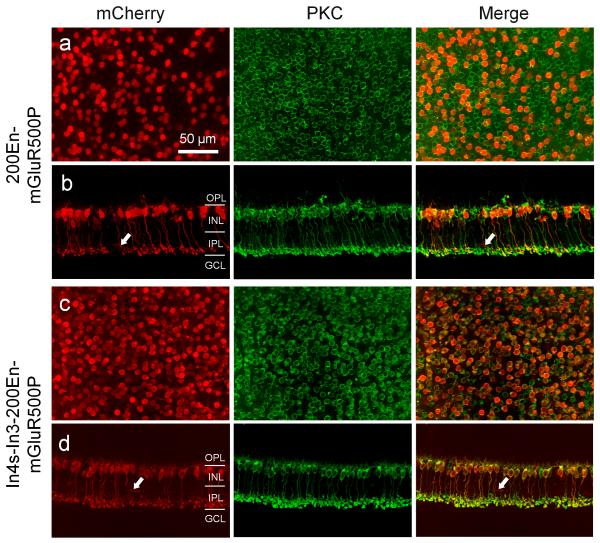
\includegraphics[width=0.52\textwidth]{Lu2016-Fig04.jpg}
\caption{图2\quad 论文原图（Lu et al., 2016）：目的基因表达产物（红）与双极细胞标记物（绿）的重叠情况}
\end{figure}

\begin{qbox}
\noindent\textbf{\color{deepgreen}第 16—18 问（据材料四作答）}
\begin{enumerate}[leftmargin=2.2em,itemsep=5pt,start=16]
\item \lv{编号选填+简答} \pt{3}
\begin{enumerate}[label=(\arabic*),leftmargin=1.4em,itemsep=2pt]
\item 若要使目的基因\textbf{主要在双极细胞中表达}，应选择表2 中的方案\tian{0.8cm}（填"甲""乙"或"丙"）（1 分）
\item 说明你的判断理由（2 分）。
\end{enumerate}

\item \lv{多选} \pt{2} 关于 AAV 载体与调控元件，下列说法正确的有（\quad）（错选得 0 分）\\
\choice{A. AAV 的作用是把目的基因送入细胞，属于基因工程中的载体\\
B. 调控元件能影响目的基因在哪些细胞中表达以及表达量的高低\\
C. 只要提高 ChR2 的总表达量，就一定能提高视觉恢复效果\\
D. 目的基因若在非目标细胞中大量表达，可能干扰视网膜原有的信号处理}

\item \lv{拔高} \pt{3} 表2 中甲方案的 ChR2 总表达量最高，但研究者并未选择它。请结合表1—表3，说明为什么"ChR2 表达量高"不能说明视觉恢复效果好。
\end{enumerate}
\end{qbox}

\section{材料五\quad 用视动反应（OMR）评价视觉功能是否恢复}
\addcontentsline{toc}{section}{材料五：用视动反应评价视觉功能}

\begin{matbox}{材料五\quad 用视动反应（OMR）评价视觉功能是否恢复}
细胞"对光有反应"不等于动物"看得见"。为评价视觉功能是否真正恢复，研究者使用\textbf{视动反应（OMR）}：把小鼠放在能显示移动条纹的装置中，若小鼠能看清条纹，其头部会随条纹运动方向转动；条纹越密集（\textbf{空间频率}越高），看清越困难，需要的光也越强。

研究者把三种 ChR2 变体分别导入三组同种失明小鼠，并设置一组\textbf{未经基因治疗}的小鼠作对照，测定了各组出现 OMR 所需的最低光强（表3）。
\end{matbox}

\begin{table}[H]
\centering\small
\caption*{\textbf{表3}\quad 各组小鼠出现 OMR 所需的最低光强（\key{命题简化}数据；"未出现"表示该条件下测不到 OMR）}
\begin{tabular}{@{}lccc@{}}
\toprule
\textbf{组别} & \textbf{条纹稀疏} & \textbf{条纹中等} & \textbf{条纹密集} \\
\midrule
未经基因治疗的对照组 & 未出现 & 未出现 & 未出现 \\
wt-ChR2 组 & 25 & 未出现 & 未出现 \\
M1 组 & 12 & 20 & 28 \\
M2 组 & 5 & 8 & 40 \\
M3 组 & 6 & 14 & 未出现 \\
\bottomrule
\end{tabular}
\end{table}

\begin{qbox}
\noindent\textbf{\color{deepgreen}第 19—21 问（据材料五作答）}
\begin{enumerate}[leftmargin=2.2em,itemsep=5pt,start=19]
\item \lv{单选} \pt{2} 在条纹稀疏与中等两种条件下，出现 OMR 所需最低光强最小（最容易被测到 OMR）的一组是（\quad）\\
\choice{A. wt-ChR2 组 \quad B. M1 组 \quad C. M2 组 \quad D. M3 组}

\item \lv{多选} \pt{2} 关于该实验，下列说法正确的有（\quad）（错选得 0 分）\\
\choice{A. 设置未经基因治疗的对照组，可用于排除其他因素引起 OMR 的可能\\
B. 各组小鼠的遗传背景、载体注射量与测定时间应保持一致\\
C. 视网膜中 ChR2 表达量越高，说明视觉恢复效果一定越好\\
D. OMR 是否出现属于行为学指标，比单纯检测蛋白表达更能反映视觉功能}

\item \lv{中等} \pt{3} 请回答下列两个问题：
\begin{enumerate}[label=(\arabic*),leftmargin=1.4em,itemsep=2pt]
\item \pt{2} 若研究目的是"比较两种 ChR2 突变体对视觉恢复的影响"，请写出该实验的\textbf{自变量}、\textbf{因变量}，以及至少两个需要控制相同的变量。
\item \pt{1} 为什么必须设置"未经基因治疗"的对照组？若该对照组也出现了 OMR，最可能说明什么？
\end{enumerate}
\end{enumerate}
\end{qbox}

\section{综合题}
\addcontentsline{toc}{section}{综合题}

\begin{qbox}
\noindent\textbf{\color{deepgreen}第 22 问（综合全部材料作答）}
\begin{enumerate}[leftmargin=2.2em,itemsep=5pt,start=22]
\item \lv{拔高·开放} \pt{3} 有一位患者以\textbf{夜间活动为主}，且需要\textbf{躲避快速移动的物体}。请综合表1—表3 的结果，从"\textbf{变体选择}、\textbf{靶细胞表达}、\textbf{功能评价}"中至少两个方面提出你的方案，并说明依据。
\end{enumerate}
\end{qbox}

\clearpage
\section*{参考答案与评分细则}
\addcontentsline{toc}{section}{参考答案与评分细则}

\begin{longtable}{@{}p{0.85cm}p{9.7cm}p{4.2cm}@{}}
\toprule
\textbf{题} & \textbf{参考答案} & \textbf{评分点} \\
\midrule
\endhead
Q1 & \textbf{A}。 & 选 A 得 2 分，其余 0 分。 \\
\addlinespace
Q2 & \textbf{①→②→④→③→⑤}。 & 完全正确得 2 分；错误或漏项 0 分。视神经由神经节细胞轴突构成，故④在③之前。 \\
\addlinespace
Q3 & \textbf{ABC}。D 错：感光细胞把光信号转变为电信号，本身就是信号加工的第一步，视网膜并非只起传递作用。 & 选 ABC 得 2 分；选两项得 1 分；含 D 得 0 分。 \\
\addlinespace
Q4 & \textbf{ABC}。D 错：细胞产生兴奋只是形成视觉的必要条件之一，还需沿完整通路传到大脑皮层并经中枢处理（材料五亦显示"细胞有反应"不等于"测得 OMR"）。 & 选 ABC 得 2 分；选两项得 1 分；含 D 得 0 分。 \\
\addlinespace
Q5 & 感光细胞是视网膜形成视觉信号的\textbf{第一站}，其功能是把光信号转变为电信号；感光细胞逐渐死亡后，光信号无法被转换，位于其下游的双极细胞、神经节细胞虽然存活却\textbf{得不到输入}，视网膜不能向大脑输出神经冲动，因此视力不断下降直至失明。 & 说出感光细胞的功能 1 分；指出信号在视网膜第一站中断 1 分；体现"下游细胞存活但无输入"1 分。仅答"细胞死了"不得分。 \\
\addlinespace
Q6 & \textbf{ABC}。D 错：需要通道蛋白协助、顺浓度梯度、不耗能的运输方式是协助扩散，不是主动运输。 & 选 ABC 得 2 分；选两项得 1 分；含 D 得 0 分。 \\
\addlinespace
Q7 & \textbf{ABC}。D 错：效应器表现出反应也可能由直接刺激引起，只有沿完整反射弧完成的反应才叫反射。 & 选 ABC 得 2 分；选两项得 1 分；含 D 得 0 分。 \\
\addlinespace
Q8 & 因为 RP 患者的\textbf{感光细胞已经大量死亡}，无法通过修复它们来恢复光感受；而位于其下游的双极细胞、神经节细胞\textbf{大多存活，且正处于视觉信号通路上}。把 ChR2 导入这些细胞后，光照可直接使它们产生电信号，从而\textbf{绕过已经死亡的感光细胞}，让信号沿原有通路继续传向大脑。 & 指出感光细胞已死亡、不能作为靶细胞 1 分；指出应选择存活且位于视觉通路上的细胞 1 分；说明可绕过死亡环节并利用原有通路 1 分。 \\
\addlinespace
Q9 & 这些细胞获得了\textbf{对光产生反应（光响应）的能力}：蓝光照射时，细胞膜上的 ChR2 通道开放，离子流入细胞，使\textbf{膜电位发生改变}，细胞由此产生电信号——即把光信号转变为电信号。\textbf{意义}：光照可以在视网膜内直接产生神经信号，绕过已死亡的感光细胞，沿原有通路传向大脑，使动物恢复对光的反应和部分视觉功能。 & 说明"通道开放→离子流动→膜电位改变→产生电信号"2 分；说明对视觉功能的意义 1 分。 \\
\addlinespace
Q10 & \textbf{ABD}。C 错：光遗传学并未修复致病基因，而是让残存细胞获得光响应能力，属于功能补偿，不是根治。 & 选 ABD 得 2 分；选两项得 1 分；含 C 得 0 分。 \\
\addlinespace
Q11 & \textbf{B}（基因突变）。基因中碱基序列发生改变引起的变异属于基因突变；题干只涉及 ChR2 基因内部碱基序列的改变，不涉及基因重组或染色体变异。 & 选 B 得 2 分；其余 0 分。 \\
\addlinespace
Q12 & 因为\textbf{基因决定蛋白质}：基因中的碱基序列决定蛋白质的氨基酸序列，氨基酸序列决定蛋白质的空间结构，而\textbf{结构决定功能}。所以通过改变基因中特定位置的碱基序列，就能改变蛋白质的氨基酸序列与空间结构，从而改变它的功能——这正是蛋白质工程的基本思路。 & 答出"基因（碱基序列）决定蛋白质的氨基酸序列"1 分；答出"结构决定功能，故改造基因即可改造蛋白质功能"1 分。 \\
\addlinespace
Q13 & M2 $>$ M3 $>$ M1 $>$ wt-ChR2。 & 完全正确得 2 分；错误或漏项 0 分。 \\
\addlinespace
Q14 & \textbf{ACD}。B 错：表1 显示被弱光激活能力越强的变体，恢复到静息所需时间越长，二者关系相反；D 对：二者总体相关但并非严格对应（M3 所需光强略高于 M2，恢复时间却更长）。 & 选 ACD 得 2 分；选两项得 1 分；含 B 得 0 分。 \\
\addlinespace
Q15 & \textbf{优势}：该突变体引起光响应所需的光强最低，在很弱的光下即可被激活，适合弱光环境（夜间、室内）。\textbf{局限}：光照停止后恢复到静息所需时间最长，对随时间快速变化的光信号（快速闪烁、运动）跟随能力最差，动态视觉信息可能难以分辨。\textbf{结论}：被弱光激活的能力强只意味着"更容易被激活"，视觉恢复还要求能分辨随时间变化的信息，故"最强"不等于"最好"，需在多指标间权衡。 & 优势 1 分；局限 1 分；得出"需权衡、最强≠最好"1 分。只答"它更敏感"不得分。 \\
\addlinespace
Q16 & (1) \textbf{丙}。(2) 丙方案在目标细胞（双极细胞）中的表达比例最高、在非目标细胞中表达极少，说明目的基因被尽量限制在双极细胞中表达，\textbf{细胞特异性最好}；甲方案虽然总表达量最高，但在非目标细胞中表达明显，不能达到"主要在双极细胞中表达"的目的。 & (1) 填"丙"1 分。(2) "双极细胞中表达比例最高"1 分；"非目标细胞中表达极少（特异性好）"或"指出甲的高表达量不等于特异性"1 分。 \\
\addlinespace
Q17 & \textbf{ABD}。C 错：总表达量提高只说明产生了更多 ChR2 蛋白，若表达在非目标细胞中或蛋白功能（如恢复时间）不合适，视觉恢复效果未必更好。 & 选 ABD 得 2 分；选两项得 1 分；含 C 得 0 分。 \\
\addlinespace
Q18 & 不充分。①"ChR2 总表达量"只说明细胞内产生了多少 ChR2 蛋白，属于\textbf{蛋白质水平}的信息；② 甲方案虽总表达量最高，但在非目标细胞中表达明显（表2），这些细胞即使产生 ChR2 也未必形成有效视觉信号，还可能干扰视网膜原有的信号处理；③ 表1、表3 表明，即使表达了蛋白，若其\textbf{恢复时间过长}（如 M3），动物在行为上仍可能测不到 OMR。因此从蛋白质水平→细胞水平→行为（功能）水平存在层次差异，视觉恢复效果最终须由\textbf{行为学功能指标}评价。 & 指出表达量属蛋白质水平、为必要而非充分条件 1 分；结合表2 说明 1 分；结合表1／表3 或明确"须以行为学功能为最终标准"1 分。 \\
\addlinespace
Q19 & \textbf{C}（M2 组）。该组在条纹稀疏、中等条件下所需最低光强（5、8）均小于其他组。 & 选 C 得 2 分；其余 0 分。 \\
\addlinespace
Q20 & \textbf{ABD}。C 错：表3 显示各组都能表达 ChR2，但所需最低光强明显不同（M2 在密集条纹下反而不如 M1），说明表达量不能代表视觉功能恢复程度。 & 选 ABD 得 2 分；选两项得 1 分；含 C 得 0 分。 \\
\addlinespace
Q21 & (1) \textbf{自变量}：导入的 ChR2 变体种类（并设未经基因治疗的对照组）；\textbf{因变量}：是否出现 OMR、出现 OMR 所需的最低光强；\textbf{需控制相同的变量}（答两个）：小鼠的遗传背景与生理状态、注射的载体量与浓度、注射后至测定的时间、条纹移动速度与光刺激条件。(2) 对照用于排除"失明小鼠自身残留的光感受能力、注射操作或光刺激"等因素引起 OMR 的可能，说明观察到的 OMR 确实由导入的 ChR2 引起；若对照组也出现 OMR，则说明该反应不是（或不只是）由 ChR2 引起——可能小鼠并未真正失去光感受能力（模型不纯）或判定标准过宽，应先检验模型、重设判定标准后再作结论。 & (1) 自变量 1 分（须含对照）；因变量 0.5 分；控制变量两个 0.5 分。(2) 对照作用 0.5 分；指出"并非由 ChR2 引起／模型不纯"0.5 分。 \\
\addlinespace
Q22 & \textbf{（示例，答出"两个方面＋依据"即可）}\newline
\textbf{① 变体选择}：夜间活动需要弱光下即可被激活，表3 中 M2 在条纹稀疏、中等时所需光强最低（5、8）；但 M2 恢复到静息所需时间最长，在条纹密集（对应快速移动物体）时所需光强反而高于 M1（40 与 28），说明它分辨快速移动物体的能力较弱。若最看重夜间看清环境可选 M2，若最看重辨识快速移动物体可考虑 M1。\newline
\textbf{② 靶细胞表达}：选择表2 中丙（或乙）方案，使 ChR2 尽量只在双极细胞中表达，减少非目标细胞表达及其对原有信号的干扰。\newline
\textbf{③ 功能评价}：不能只用一种条件评价疗效，应同时测定条纹稀疏与密集条件下的 OMR，并增加如瞳孔对光收缩等其他指标。\newline
\textbf{结论}：视觉恢复需综合考虑被弱光激活的能力、恢复时间、靶细胞表达、非目标细胞表达以及行为水平的功能表现。 & 结合"夜间（弱光）"与"移动物体（快速变化）"两个需求并引用表3 数据 1 分；指出 M2 与 M1 的取舍关系 1 分；从至少两个方面提出方案且合理 0.5 分；得出"需综合多指标"的结论 0.5 分。 \\
\bottomrule
\end{longtable}

\section*{命题底线自检}
\addcontentsline{toc}{section}{命题底线自检}

\begin{longtable}{@{}p{0.6cm}p{6.0cm}p{8.2cm}@{}}
\toprule
\textbf{\#} & \textbf{底线要求} & \textbf{落实情况} \\
\midrule
\endhead
1 & 不要求学生背诵 ChR2、mGluR6、AAV 的专业定义 & 均以"材料给定的含义"出现；选择题只考其\emph{功能角色}，不考定义式记忆。 \\
\addlinespace
2 & 首次出现的专业事实必须给出必要解释 & 视网膜各级细胞分工见材料一与图1；ChR2 的性质与作用方式见材料二；蛋白质工程思路（结构与功能的关系、改造基因以改造蛋白）见材料三；AAV 与调控元件见材料四；OMR 与空间频率见材料五。 \\
\addlinespace
3 & 不使用大学电生理学作为直接考点 & 神经系统题只考教材层面的"电信号传导、突触单向传递、视神经为传入神经、反射与反射弧"；未要求解释动作电位的离子机制。 \\
\addlinespace
4 & 不要求记忆实验编号、载体编号、品系名称 & 全文无载体编号、血清型与小鼠品系名称（变体以 M1—M3 代号出现，含义已在表1 注明）。 \\
\addlinespace
5 & 专业数据经过高中化处理 & 表1—表3 均为相对值并标注"命题简化"，趋势依原文改写。 \\
\addlinespace
6 & 高难度来自多证据整合 & Q15（表1 两列指标权衡）、Q18（表1＋表2＋表3 整合）、Q22（五段材料整合）难点均在证据整合与变量分析。 \\
\addlinespace
7 & 每个结论都有材料或高中知识支持 & 逐问核查：Q1—Q5（图1＋材料一）、Q6—Q10（材料二＋教材膜运输与反射弧知识）、Q11—Q15（材料三＋表1）、Q16—Q18（表2＋图2）、Q19—Q21（表3）、Q22（前文全部）。 \\
\bottomrule
\end{longtable}

\section*{附录\quad 论文原图对照（课堂延伸用）}
\addcontentsline{toc}{section}{附录：论文原图对照}

\begin{figure}[H]
\centering
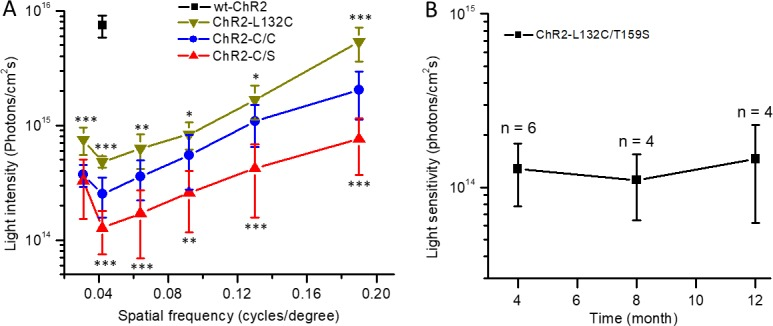
\includegraphics[width=0.68\textwidth]{Lu2018-Fig04.jpg}
\caption{图A\quad 论文原图（Lu et al., \textit{IOVS}, 2018, Fig.~4）：三种 ChR2 变体的 OMR 阈值光强—空间频率关系，与表3 的设计思路一致，供课堂延伸或按真实数据替换表3 时对照使用。}
\end{figure}

\noindent\small 全部 22 张论文原图与三篇文献存于 \texttt{00 - Personal/Resources/Downloads/}。

\end{document}
